\subsection{Specifica componenti Model::Core::Algorithm}
\label{specificaModelCoreAlgorithm}

\begin{figure}[!h]
\centering
			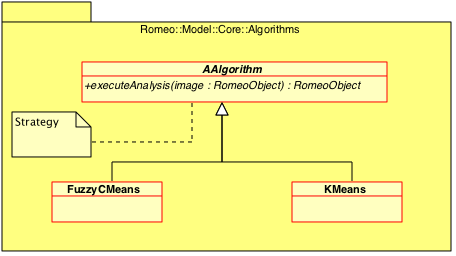
\includegraphics[scale=1]{../Specifica_Tecnica/Content/Immagini/Romeo__Model__Core__Adapters__Algorithms.png}
			\caption{Componente Romeo::Model::Core::Algorithm}
			\label{romeo_model_core}
\end{figure}

Package\g{} contenente le classi per gli algoritmi di clustering\g{}.
% % % % % % % % % % % % % % % % % % % % % %
% % % % AAlgorithm
% % % % % % % % % % % % % % % % % % % %
\subsubsection{AAlgorithm (abstract)}
\label{aalgorithm}
\begin{figure}[!h]
\centering
			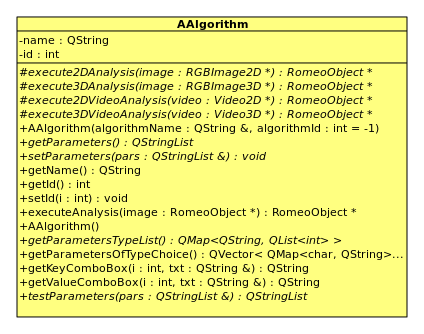
\includegraphics[scale=1]{./Content/Immagini/modelCore/AAlgorithm.png}
			\caption{Diagramma classe \textsl{AAlgorithm}}
			\label{aalgorithm_img}
\end{figure}

\paragraph{Descrizione \\} Classe astratta che rappresenta un generico algoritmo di clustering\g{}, secondo il design pattern Strategy. Definisce dei contratti per l'esecuzione degli algoritmi, che dovranno essere implementati dalle sue sottoclassi.

\paragraph{Utilizzo\\} Fornisce i metodi per l'esecuzione di un algoritmo di clustering su un immagine bidimensionale o tridimensionale.

\paragraph{Attributi\\}
	\begin{itemize}
		\item  \color{teal}\verb! - name : QString !\\
		\color{black}
		\subparagraph{Descrizione:} nome dell'algoritmo.
		\item  \color{teal}\verb! - id : int !\\
		\color{black}
		\subparagraph{Descrizione:} codice identificativo dell'algoritmo.
	\end{itemize}
	
\paragraph{Metodi\\}
	\begin{itemize}
		\item \color{blue}\verb! # execute2DAnalysis(image :RGBImage2D*) : RomeoObject* !\\
			\color{black}
			\subparagraph{Descrizione:} metodo che esegue l'algoritmo di clustering su un immagine bidimensionale.
			\subparagraph{Argomenti}
				\begin{itemize}
					\item \color{RoyalPurple}\verb!image : RGBImage2D*!\\
					\color{black} immagine bidimensionale su cui eseguire l'algoritmo di clustering.
				\end{itemize}
				\subparagraph{Note}
				\begin{itemize}
					\item il metodo deve essere marcato virtuale puro.
				\end{itemize}
				
		\item \color{blue}\verb! # execute3DAnalysis(image :RGBImage3D*) : RomeoObject* !\\
			\color{black}
			\subparagraph{Descrizione:} metodo che esegue l'algoritmo di clustering su un immagine tridimensionale.
			\subparagraph{Argomenti}
				\begin{itemize}
					\item \color{RoyalPurple}\verb!image : RGBImage3D*!\\
					\color{black} immagine tridimensionale su cui eseguire l'algoritmo di clustering.
				\end{itemize}
				\subparagraph{Note}
				\begin{itemize}
					\item il metodo deve essere marcato virtuale puro.
				\end{itemize}
				
		\item \color{blue}\verb! # execute2DVideoAnalysis(video :Video2D*) : RomeoObject* !\\
			\color{black}
			\subparagraph{Descrizione:} metodo che esegue l'algoritmo di clustering su un video bidimensionale.
			\subparagraph{Argomenti}
				\begin{itemize}
					\item \color{RoyalPurple}\verb!video ; Video2D* !\\
					\color{black} video bidimensionale su cui eseguire l'algoritmo di clustering.
				\end{itemize}
				\subparagraph{Note}
				\begin{itemize}
					\item il metodo deve essere marcato virtuale puro.
				\end{itemize}
		\item \color{blue}\verb! # execute3DVideoAnalysis(video : Video3D*) : RomeoObject* !\\
			\color{black}
			\subparagraph{Descrizione:} metodo che esegue l'algoritmo di clustering su un video tridimensionale.
			\subparagraph{Argomenti}
				\begin{itemize}
					\item \color{RoyalPurple}\verb!image : RGBImage2D*!\\
					\color{black} video tridimensionale su cui eseguire l'algoritmo di clustering.
				\end{itemize}
				\subparagraph{Note}
			\begin{itemize}
				\item il metodo deve essere marcato virtuale puro.
			\end{itemize}
			
		\item \color{blue}\verb! + AAlgorithm(algorithmName : const QString& ,algorithmId : int)!\\
			\color{black}
			\subparagraph{Descrizione:} costruttore della classe.
			\subparagraph{Argomenti}
				\begin{itemize}
					\item \color{RoyalPurple}\verb!algorithmName : const QString& !\\
					\color{black} nome dell'algoritmo.
					\item \color{RoyalPurple}\verb!algorithmId : int!\\
					\color{black} codice identificativo dell'algoritmo.
				\end{itemize}
			
	\item \color{blue}\verb! + getParameters() : QStringList!
		\color{black}
		\subparagraph{Descrizione:} metodo che ritorna la lista dei parametri dell'algoritmo di clustering\g{} .
		\subparagraph{Note}
			\begin{itemize}
				\item il metodo deve essere marcato virtuale.
				\item il metodo deve essere marcato cost.
			\end{itemize}
			
	\item \color{blue}\verb! + setParameters(params : const QStringList &) : void!
		\color{black}
		\subparagraph{Descrizione:} inserisce i parametri dell'algoritmo di clustering\g{}.
		\subparagraph{Argomenti}
			\begin{itemize}
				\item \color{RoyalPurple} \verb!params : const QStringList & ! \\ 
				\color{black} lista di parametri dell'algoritmo di clustering\g{}..		
			\end{itemize}
		\subparagraph{Note}
			\begin{itemize}
				\item il metodo deve essere marcato virtuale.
			\end{itemize}
			
	\item \color{blue}\verb! + getName() : QString!
		\color{black}
		\subparagraph{Descrizione:} metodo che ritorna il nome dell'algoritmo di clustering\g{} .
		\subparagraph{Note}
			\begin{itemize}
				\item il metodo deve essere marcato virtuale.
				\item il metodo deve essere marcato cost.
			\end{itemize}
			
	\item \color{blue}\verb! + getId() :int!
		\color{black}
		\subparagraph{Descrizione:} metodo che ritorna il codice identificativo dell'algoritmo di clustering\g{} .
		\subparagraph{Note}
			\begin{itemize}
				\item il metodo deve essere marcato cost.
			\end{itemize}
				
	\item \color{blue}\verb! + setId(i : int) : void!
		\color{black}
		\subparagraph{Descrizione:} inserisce il codice identificativo dell'algoritmo di clustering\g{}.
		\subparagraph{Argomenti}
			\begin{itemize}
				\item \color{RoyalPurple} \verb!i : int ! \\ 
				\color{black} codice identificativo dell'algoritmo di clustering\g{}..		
			\end{itemize}
		
			
	\item \color{blue}\verb! + executeAnalysis(image : RomeoObject* ) : RomeoObject*!
		\color{black}
		\subparagraph{Descrizione:} esegue l'algoritmo di clustering\g{} su un generico dato.
		\subparagraph{Argomenti}
			\begin{itemize}
				\item \color{RoyalPurple} \verb!image : RomeoObject* ! \\ 
				\color{black} generico dato su cui applicare l'algoritmo di clustering\g{}..		
			\end{itemize}
			
	\item \color{blue}\verb! + AAlgorithm()!
		\color{black}
		\subparagraph{Descrizione:} costruttore di default.
			
	\item \color{blue}\verb! + getParametersTypeList()  : QMap<QString, QList<int> >!
		\color{black}
		\subparagraph{Descrizione:} metodo che ritorna la lista dei parametri di tipo dell'algoritmo di clustering\g{} .
		\subparagraph{Note}
			\begin{itemize}
				\item il metodo deve essere marcato virtuale puro.
				\item il metodo deve essere marcato costante.
			\end{itemize}	
			
	\item \color{blue}\verb! + getParametersOfTypeChoice()  : QVector< QMap<char, QString> >!
		\color{black}
		\subparagraph{Descrizione:} metodo che ritorna la lista dei parametri di scelta dell'algoritmo di clustering\g{} .
		\subparagraph{Note}
			\begin{itemize}
				\item il metodo deve essere marcato virtuale.
				\item il metodo deve essere marcato costante.
			\end{itemize}	
	
	\item \color{blue}\verb! + getKeyComboBox(i : int , txt : const QString & ) : QString!
		\color{black}
		\subparagraph{Descrizione:} metodo che ritorna la lista delle chaivi combobox.
		\subparagraph{Argomenti}
			\begin{itemize}
				\item \color{RoyalPurple} \verb!i : int ! \\ 
				\color{black} indice combobox.
				\item \color{RoyalPurple} \verb!txt : const QString & ! \\ 
				\color{black} valore combobox.		
			\end{itemize}
		\subparagraph{Note}
			\begin{itemize}
				\item il metodo deve essere marcato virtuale.
				\item il metodo deve essere marcato costante.
			\end{itemize}	
			
	\item \color{blue}\verb! + getValueComboBox(i : int , txt : const QString & ) : QString!
		\color{black}
		\subparagraph{Descrizione:} metodo che ritorna la lista del valori del combobox.
		\subparagraph{Argomenti}
			\begin{itemize}
				\item \color{RoyalPurple} \verb!i : int ! \\ 
				\color{black} indice combobox.
				\item \color{RoyalPurple} \verb!txt : const QString & ! \\ 
				\color{black} valore combobox.		
			\end{itemize}
		\subparagraph{Note}
			\begin{itemize}
				\item il metodo deve essere marcato virtuale .
				\item il metodo deve essere marcato costante.
			\end{itemize}				
			
		\item \color{blue}\verb! + testParameters(pars : const QStringList &) : QStringList!
		\color{black}
		\subparagraph{Descrizione:} metodo che ritorna la lista il test dei parametri.
		\subparagraph{Argomenti}
			\begin{itemize}
				\item \color{RoyalPurple} \verb!pars : const QStringList & ! \\ 
				\color{black} valore dei parametri.	
			\end{itemize}
		\subparagraph{Note}
			\begin{itemize}
				\item il metodo deve essere marcato virtuale puro .
				\item il metodo deve essere marcato costante.
			\end{itemize}				
			
	\end{itemize}
\pagebreak
% % % % % % % % % % % % % % % % % % % % % % % % % % % % % % % % 
% % % FUZZYCMEANALGORITHM% % % % % % % % % % % % % % % % % % % %
% % % % % % % % % % % % % % % % % % % % % % % % % % % % % % % % %
\color{black}
\subsubsection{FuzzyCMeansAlgorithm (class)}
\label{fuzzyCMeansAlgorithm}
\begin{figure}[!h]
\centering
			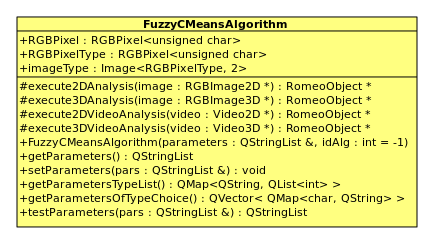
\includegraphics[scale=1]{./Content/Immagini/modelCore/FuzzyCMeansAlgorithm.png}
			\caption{Diagramma classe \textsl{FuzzyCMeansAlgorithm}}
			\label{fuzzyCMeansAlgorithm_img}
\end{figure}

\paragraph{Descrizione \\} Classe che implementa l'algoritmo di clustering\g{} \textit{FuzzyCMeans}.

\paragraph{Utilizzo\\} Viene utilizzata durante un'analisi per applicare l'algoritmo a un \dataset{}.

\paragraph{Eredita da:}
\begin{itemize}
	\item AAlgorithm.
\end{itemize}


	
\paragraph{Metodi\\}
	\begin{itemize}
		\item \color{blue}\verb! # execute2DAnalysis(image :RGBImage2D*) : RomeoObject* !\\
			\color{black}
			\subparagraph{Descrizione:} metodo che esegue l'algoritmo di clustering su un immagine bidimensionale.
			\subparagraph{Argomenti}
				\begin{itemize}
					\item \color{RoyalPurple}\verb!image : RGBImage2D*!\\
					\color{black} immagine bidimensionale su cui eseguire l'algoritmo di clustering.
				\end{itemize}
				\subparagraph{Note}
				\begin{itemize}
					\item il metodo deve essere marcato virtuale.
				\end{itemize}
				
		\item \color{blue}\verb! # execute3DAnalysis(image :RGBImage3D*) : RomeoObject* !\\
			\color{black}
			\subparagraph{Descrizione:} metodo che esegue l'algoritmo di clustering su un immagine tridimensionale.
			\subparagraph{Argomenti}
				\begin{itemize}
					\item \color{RoyalPurple}\verb!image : RGBImage3D*!\\
					\color{black} immagine tridimensionale su cui eseguire l'algoritmo di clustering.
				\end{itemize}
				\subparagraph{Note}
				\begin{itemize}
					\item il metodo deve essere marcato virtuale.
				\end{itemize}
				
		\item \color{blue}\verb! # execute2DVideoAnalysis(video :Video2D*) : RomeoObject* !\\
			\color{black}
			\subparagraph{Descrizione:} metodo che esegue l'algoritmo di clustering su un video bidimensionale.
			\subparagraph{Argomenti}
				\begin{itemize}
					\item \color{RoyalPurple}\verb!video ; Video2D* !\\
					\color{black} video bidimensionale su cui eseguire l'algoritmo di clustering.
				\end{itemize}
				\subparagraph{Note}
				\begin{itemize}
					\item il metodo deve essere marcato virtuale.
				\end{itemize}
		\item \color{blue}\verb! # execute3DVideoAnalysis(video : Video3D*) : RomeoObject* !\\
			\color{black}
			\subparagraph{Descrizione:} metodo che esegue l'algoritmo di clustering su un video tridimensionale.
			\subparagraph{Argomenti}
				\begin{itemize}
					\item \color{RoyalPurple}\verb!image : RGBImage2D*!\\
					\color{black} video tridimensionale su cui eseguire l'algoritmo di clustering.
				\end{itemize}
				\subparagraph{Note}
			\begin{itemize}
				\item il metodo deve essere marcato virtuale.
			\end{itemize}
			
		\item \color{blue}\verb! + FuzzyCMeansAlgorithm(parameters : StringList & ,idAlg : int)!\\
			\color{black}
			\subparagraph{Descrizione:} costruttore della classe.
			\subparagraph{Argomenti}
				\begin{itemize}
					\item \color{RoyalPurple}\verb!parameters:  StringList &  !\\
					\color{black} parametri dell'algoritmo.
					\item \color{RoyalPurple}\verb!idAlg : int!\\
					\color{black} codice identificativo dell'algoritmo.
				\end{itemize}
			
	\item \color{blue}\verb! + getParameters() : QStringList!
		\color{black}
		\subparagraph{Descrizione:} metodo che ritorna la lista dei parametri dell'algoritmo di clustering\g{} .
		\subparagraph{Note}
			\begin{itemize}
				\item il metodo deve essere marcato virtuale.
				\item il metodo deve essere marcato cost.
			\end{itemize}
			
	\item \color{blue}\verb! + setParameters(params : const QStringList &) : void!
		\color{black}
		\subparagraph{Descrizione:} inserisce i parametri dell'algoritmo di clustering\g{}.
		\subparagraph{Argomenti}
			\begin{itemize}
				\item \color{RoyalPurple} \verb!params : const QStringList & ! \\ 
				\color{black} lista di parametri dell'algoritmo di clustering\g{}..		
			\end{itemize}
		\subparagraph{Note}
			\begin{itemize}
				\item il metodo deve essere marcato virtuale.
			\end{itemize}
					
	\item \color{blue}\verb! + getParametersTypeList()  : QMap<QString, QList<int> >!
		\color{black}
		\subparagraph{Descrizione:} metodo che ritorna la lista dei parametri di tipo dell'algoritmo di clustering\g{} .
		\subparagraph{Note}
			\begin{itemize}
				\item il metodo deve essere marcato virtuale.
				\item il metodo deve essere marcato costante.
			\end{itemize}	
			
	\item \color{blue}\verb! + getParametersOfTypeChoice()  : QVector< QMap<char, QString> >!
		\color{black}
		\subparagraph{Descrizione:} metodo che ritorna la lista dei parametri di scelta dell'algoritmo di clustering\g{} .
		\subparagraph{Note}
			\begin{itemize}
				\item il metodo deve essere marcato virtuale.
				\item il metodo deve essere marcato costante.
			\end{itemize}	
	
		\item \color{blue}\verb! + testParameters(pars : const QStringList &) : QStringList!
		\color{black}
		\subparagraph{Descrizione:} metodo che ritorna la lista il test dei parametri.
		\subparagraph{Argomenti}
			\begin{itemize}
				\item \color{RoyalPurple} \verb!pars : const QStringList & ! \\ 
				\color{black} valore dei parametri.	
			\end{itemize}
		\subparagraph{Note}
			\begin{itemize}
				\item il metodo deve essere marcato virtuale.
				\item il metodo deve essere marcato costante.
			\end{itemize}				
			
	\end{itemize}
\pagebreak
% % % % % % % % % % % % % % % % % % % % % % % % % % % % % % % % %
% % % % % % K MEANS ALGORITHM% % % % % % % % % % % % % % % % % % % % % % %
% % % % % % % % % % % % % % % % % % % % % % % % % % % % % %
\color{black}
\subsubsection{KMeansAlgorithm (class)}
\label{KMeanslAlgorithm}
\begin{figure}[!h]
\centering
			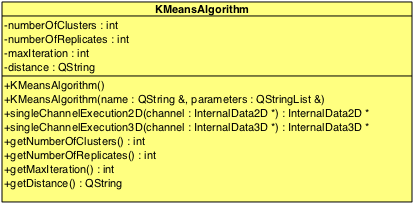
\includegraphics[scale=1]{./Content/Immagini/modelCore/KMeansAlgorithm.png}
			\caption{Diagramma classe \textsl{KMeansAlgorithm}}
			\label{KMeansAlgorithm_img}
\end{figure}

\paragraph{Descrizione \\} Classe che implementa l'algoritmo di clustering\g{} \textit{KMeans}.

\paragraph{Utilizzo\\} Viene utilizzata durante un'analisi per applicare l'algoritmo a un \dataset{}.

\paragraph{Eredita da:}
\begin{itemize}
	\item AAlgorithm.
\end{itemize}

\paragraph{Attributi\\}
	\begin{itemize}
		\item  \color{teal}\verb! - numberOfCluster : int !\\
		\color{black}
		\subparagraph{Descrizione:} Numero dei cluster per l'applicazione dell'algoritmo.
		\item  \color{teal}\verb! - numberOfReplicates : int !\\
		\color{black}
		\subparagraph{Descrizione:} Specifica il numero di volte che l'algoritmo deve essere applicato.
		\item  \color{teal}\verb! - maxIteration : int !\\
		\color{black}
		\subparagraph{Descrizione:} Limite massimo di iterazioni per l'algoritmo.
		\item  \color{teal}\verb! - distance : QString !\\
		\color{black}
		\subparagraph{Descrizione:} Tipo di distanza per l'applicazione dell'algoritmo.
	\end{itemize}
	
\paragraph{Metodi\\}
	\begin{itemize}
		\item \color{blue}\verb! # execute2DAnalysis(image :RGBImage2D*) : RomeoObject* !\\
			\color{black}
			\subparagraph{Descrizione:} metodo che esegue l'algoritmo di clustering su un immagine bidimensionale.
			\subparagraph{Argomenti}
				\begin{itemize}
					\item \color{RoyalPurple}\verb!image : RGBImage2D*!\\
					\color{black} immagine bidimensionale su cui eseguire l'algoritmo di clustering.
				\end{itemize}
				\subparagraph{Note}
				\begin{itemize}
					\item il metodo deve essere marcato virtuale.
				\end{itemize}
				
		\item \color{blue}\verb! # execute3DAnalysis(image :RGBImage3D*) : RomeoObject* !\\
			\color{black}
			\subparagraph{Descrizione:} metodo che esegue l'algoritmo di clustering su un immagine tridimensionale.
			\subparagraph{Argomenti}
				\begin{itemize}
					\item \color{RoyalPurple}\verb!image : RGBImage3D*!\\
					\color{black} immagine tridimensionale su cui eseguire l'algoritmo di clustering.
				\end{itemize}
				\subparagraph{Note}
				\begin{itemize}
					\item il metodo deve essere marcato virtuale.
				\end{itemize}
				
		\item \color{blue}\verb! # execute2DVideoAnalysis(video :Video2D*) : RomeoObject* !\\
			\color{black}
			\subparagraph{Descrizione:} metodo che esegue l'algoritmo di clustering su un video bidimensionale.
			\subparagraph{Argomenti}
				\begin{itemize}
					\item \color{RoyalPurple}\verb!video ; Video2D* !\\
					\color{black} video bidimensionale su cui eseguire l'algoritmo di clustering.
				\end{itemize}
				\subparagraph{Note}
				\begin{itemize}
					\item il metodo deve essere marcato virtuale.
				\end{itemize}
		\item \color{blue}\verb! # execute3DVideoAnalysis(video : Video3D*) : RomeoObject* !\\
			\color{black}
			\subparagraph{Descrizione:} metodo che esegue l'algoritmo di clustering su un video tridimensionale.
			\subparagraph{Argomenti}
				\begin{itemize}
					\item \color{RoyalPurple}\verb!image : RGBImage2D*!\\
					\color{black} video tridimensionale su cui eseguire l'algoritmo di clustering.
				\end{itemize}
				\subparagraph{Note}
			\begin{itemize}
				\item il metodo deve essere marcato virtuale.
			\end{itemize}

		\item \color{blue}\verb! + MeansAlgorithm(idAlg : int)!\\
			\color{black}
			\subparagraph{Descrizione:} costruttore della classe a un parametro.
			\subparagraph{Argomenti}
				\begin{itemize}
					\item \color{RoyalPurple}\verb!idAlg : int!\\
					\color{black} codice identificativo dell'algoritmo.
				\end{itemize}			
		
		\item \color{blue}\verb! + MeansAlgorithm(parameters : StringList & ,idAlg : int)!\\
			\color{black}
			\subparagraph{Descrizione:} costruttore della classe.
			\subparagraph{Argomenti}
				\begin{itemize}
					\item \color{RoyalPurple}\verb!parameters:  StringList &  !\\
					\color{black} parametri dell'algoritmo.
					\item \color{RoyalPurple}\verb!idAlg : int!\\
					\color{black} codice identificativo dell'algoritmo.
				\end{itemize}
		
		\item \color{blue}\verb! + getNumberOfClusters() : int!
		\color{black}
		\subparagraph{Descrizione:} metodo che ritorna il numero di cluster dell'algoritmo di clustering\g{} .
		\subparagraph{Note}
			\begin{itemize}
				\item il metodo deve essere marcato cost.
			\end{itemize}
			
			\item \color{blue}\verb! + getNumberOfReplicates() : int!
		\color{black}
		\subparagraph{Descrizione:} metodo che ritorna il numero di replicates dell'algoritmo di clustering\g{} .
		\subparagraph{Note}
			\begin{itemize}
				\item il metodo deve essere marcato cost.
			\end{itemize}
			\item \color{blue}\verb! + getMaxIteration() : int!
		\color{black}
		\subparagraph{Descrizione:} metodo che ritorna il numero massimo di iterazioni dell'algoritmo di clustering\g{} .
		\subparagraph{Note}
			\begin{itemize}
				\item il metodo deve essere marcato cost.
			\end{itemize}
			\item \color{blue}\verb! + getDistance() : char!
		\color{black}
		\subparagraph{Descrizione:} metodo che ritorna il tipo di distanza dell'algoritmo di clustering\g{} .
		\subparagraph{Note}
			\begin{itemize}
				\item il metodo deve essere marcato cost.
			\end{itemize}
			
			
	\item \color{blue}\verb! + getParameters() : QStringList!
		\color{black}
		\subparagraph{Descrizione:} metodo che ritorna la lista dei parametri dell'algoritmo di clustering\g{} .
		\subparagraph{Note}
			\begin{itemize}
				\item il metodo deve essere marcato virtuale.
				\item il metodo deve essere marcato cost.
			\end{itemize}
			
	\item \color{blue}\verb! + setParameters(params : const QStringList &) : void!
		\color{black}
		\subparagraph{Descrizione:} inserisce i parametri dell'algoritmo di clustering\g{}.
		\subparagraph{Argomenti}
			\begin{itemize}
				\item \color{RoyalPurple} \verb!params : const QStringList & ! \\ 
				\color{black} lista di parametri dell'algoritmo di clustering\g{}..		
			\end{itemize}
		\subparagraph{Note}
			\begin{itemize}
				\item il metodo deve essere marcato virtuale.
			\end{itemize}
					
	\item \color{blue}\verb! + getParametersTypeList()  : QMap<QString, QList<int> >!
		\color{black}
		\subparagraph{Descrizione:} metodo che ritorna la lista dei parametri di tipo dell'algoritmo di clustering\g{} .
		\subparagraph{Note}
			\begin{itemize}
				\item il metodo deve essere marcato virtuale.
				\item il metodo deve essere marcato costante.
			\end{itemize}	
			
	\item \color{blue}\verb! + getParametersOfTypeChoice()  : QVector< QMap<char, QString> >!
		\color{black}
		\subparagraph{Descrizione:} metodo che ritorna la lista dei parametri di scelta dell'algoritmo di clustering\g{} .
		\subparagraph{Note}
			\begin{itemize}
				\item il metodo deve essere marcato virtuale.
				\item il metodo deve essere marcato costante.
			\end{itemize}	
	
		\item \color{blue}\verb! + testParameters(pars : const QStringList &) : QStringList!
		\color{black}
		\subparagraph{Descrizione:} metodo che ritorna la lista il test dei parametri.
		\subparagraph{Argomenti}
			\begin{itemize}
				\item \color{RoyalPurple} \verb!pars : const QStringList & ! \\ 
				\color{black} valore dei parametri.	
			\end{itemize}
		\subparagraph{Note}
			\begin{itemize}
				\item il metodo deve essere marcato virtuale.
				\item il metodo deve essere marcato costante.
			\end{itemize}				
			
	\end{itemize}
